\documentclass[11pt,a4paper]{article}   
\usepackage[left=2cm,right=2cm,top=2cm,bottom=2cm]{geometry}

\usepackage[utf8]{inputenc}
\usepackage[T1]{fontenc}


\usepackage{apacite} % Para citas en formato APA
%\usepackage[spanish, es-noquoting]{babel} % Para idioma en español
\usepackage{amsmath}  % Para matemáticas avanzadas
\usepackage{amssymb}  % Para símbolos matemáticos
\usepackage{graphicx}  % Para incluir imágenes
\usepackage{longtable} % Para tablas que se extienden por varias páginas
\usepackage{booktabs}  % Mejor formato para tablas
\usepackage{tikz}  % Para gráficos con TikZ
\usepackage{pgfplots}  % Para gráficos avanzados
\usepackage[hidelinks]{hyperref}  % Para enlaces sin bordes

\usepackage{float}
\usepackage{enumitem}
\usepackage{multicol}

 \usepackage{ragged2e} 
 
\usepackage{setspace}
\onehalfspacing  

 

 \usepackage{authblk}

\title{Diseño y Selección de Materiales para una Cámara de Refrigeración para la Conservación de Insulina en la UMF 40, Azcapotzalco, CDMX}  
\author[1]{Monjaraz Ramírez, Israel} 
\affil[1]{Instituto Politécnico Nacional, ESIME Azcapotzalco, CDMX} 
\author[2]{García Lira, Jesús}
\affil[2]{Instituto Politécnico Nacional, ESIME Azcapotzalco, Academia de Ciencia de los Materiales, CDMX}
 
\date{11 de diciembre de 2024} 

%\usepackage{lmodern} 
\usepackage{mathptmx}

\pgfplotsset{compat=1.18}
\begin{document}

\maketitle

\justifying

\section*{Resumen}
Este trabajo presenta el diseño y desarrollo de una cámara de refrigeración médica destinada a la conservación de insulina en la UMF40 Santa Bárbara, Azcapotzalco, CDMX. La selección adecuada de materiales para la construcción del equipo es crucial para garantizar un almacenamiento seguro y eficiente de la insulina. Se detallan los criterios para la elección de materiales que optimicen la eficiencia energética, el aislamiento térmico y la durabilidad del sistema. Adicionalmente, se realizarán simulaciones térmicas mediante ANSYS para evaluar el flujo de calor y las distribuciones de temperatura, garantizando un desempeño eficiente bajo diferentes condiciones de operación. Entre los enfoques de ciencia de materiales aplicados, destaca el uso de poliuretano expandido por su baja conductividad térmica y del acero inoxidable por su alta resistencia a la corrosión, ambos esenciales para mantener condiciones óptimas de temperatura y prolongar la vida útil del equipo. Estas estrategias aseguran que la cámara mantenga un ambiente estable, preservando la efectividad de la insulina incluso en escenarios críticos.


\textbf{Palabras clave:} Cámara de refrigeración, conservación de insulina, eficiencia energética, aislamiento térmico, simulación térmica, ciencia de materiales, ANSYS, poliuretano expandido, acero inoxidable, sistemas de refrigeración médica.


\section*{Abstract}
This work presents the design and development of a medical refrigeration chamber for insulin storage at UMF40 Santa Bárbara, Azcapotzalco, CDMX. The proper selection of materials for the construction of the equipment is crucial to ensure safe and efficient storage of insulin. Criteria for the selection of materials that optimize energy efficiency, thermal insulation and durability of the system are detailed. Additionally, thermal simulations will be performed using ANSYS to evaluate heat flow and temperature distributions, ensuring efficient performance under different operating conditions. Among the material science approaches applied, the use of expanded polyurethane for its low thermal conductivity and stainless steel for its high corrosion resistance, both essential for maintaining optimum temperature conditions and extending the useful life of the equipment, stand out. These strategies ensure that the chamber maintains a stable environment, preserving insulin effectiveness even in critical scenarios.

\textbf{Keywords:} Refrigeration chamber, insulin preservation, energy efficiency, thermal insulation, thermal simulation, material science, ANSYS, expanded polyurethane, stainless steel, medical refrigeration systems.


\setlength{\columnsep}{1cm}
\begin{multicols}{2}
	
\section{Introducción}
La refrigeración es un proceso fundamental para la conservación de alimentos, medicamentos y otros productos sensibles a la temperatura. Este proceso consiste en la transferencia de calor desde un espacio confinado hacia un entorno de mayor temperatura, permitiendo mantener condiciones controladas dentro del sistema. La eficiencia en la gestión térmica es crucial, ya que un diseño adecuado no solo previene el deterioro de los productos, sino que también optimiza el consumo energético, lo cual es especialmente relevante en sistemas médicos donde la fiabilidad y eficiencia son imprescindibles (\citeauthor{Dincer2010-re}, 2010)\\
En el ámbito médico, la refrigeración desempeña un papel crucial en la conservación de medicamentos como la insulina, una hormona esencial para el tratamiento de la diabetes mellitus. La insulina debe mantenerse entre $2^\circ$C y $8^\circ$C para preservar su efectividad; temperaturas fuera de este rango pueden provocar la desnaturalización de la proteína, inutilizando el medicamento y poniendo en riesgo la salud de los pacientes (\citeauthor{ashrae-about}, 2023). Este desafío es particularmente relevante en entornos de alta altitud y temperaturas extremas, donde los sistemas de refrigeración deben estar adaptados a condiciones locales para asegurar un rendimiento óptimo.\\
La Ciudad de México presenta retos particulares debido a su altitud (2250 m sobre el nivel del mar) y temperaturas promedio de $23^\circ$C. Estas condiciones afectan el diseño de los sistemas de refrigeración, ya que la presión atmosférica más baja disminuye la eficiencia de los compresores y condensadores (Kuashik, 2017). Esto resalta la necesidad de sistemas que no solo sean eficientes, sino también adaptados a las condiciones locales (\citeauthor{Dincer2010-re}, 2010).\\
Un diseño eficiente de sistemas de refrigeración para equipos médicos requiere una cuidadosa selección de materiales y el uso de simulaciones térmicas avanzadas. En particular, la ciencia de materiales desempeña un papel clave en el desarrollo de componentes como aislantes térmicos, recubrimientos internos y externos, y sellos herméticos (Dincer \& Ratlamwala, 2016). Materiales como el poliuretano expandido, con su baja conductividad térmica y alta resistencia al envejecimiento, son ideales para reducir las pérdidas térmicas (Zhang \& Eikevek, 2017). Asimismo, el uso de recubrimientos de acero inoxidable garantiza la durabilidad estructural y la resistencia a la corrosión, indispensables en entornos médicos donde los equipos deben ser capaces de soportar condiciones exigentes (Cengel, 2009).
\begin{figure}[H]
	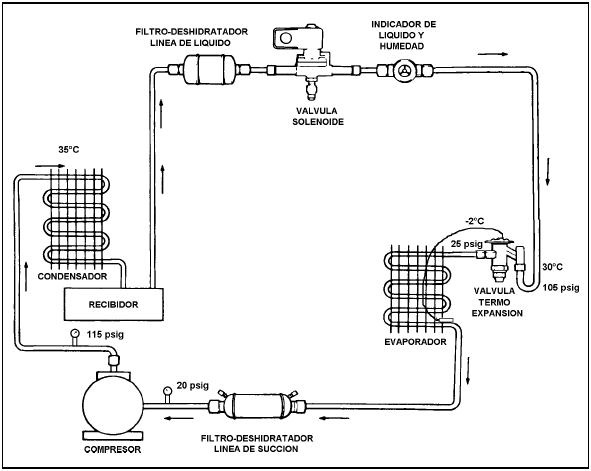
\includegraphics[width=\linewidth]{figures/ciclo-ref.png}
	\caption{Ciclo de refrigeración}
	\label{fig:ciclo}	
\end{figure} La validación de estos sistemas se realiza mediante simulaciones térmicas detalladas que evalúan el flujo de calor, las distribuciones de temperatura y el comportamiento del sistema bajo diferentes escenarios de operación. Herramientas como ANSYS permiten optimizar el diseño antes de la construcción, minimizando riesgos y garantizando el cumplimiento de normativas internacionales en equipos médicos. Estas simulaciones también identifican posibles fallas, mejorando la confiabilidad y prolongando la vida útil del equipo. El ciclo de refrigeración, representado en la Figura \ref{fig:ciclo}, es fundamental para entender cómo se realiza la transferencia de calor en este tipo de sistemas. El diagrama T-S, mostrado en la Figura \ref{fig:diag-ts}, complementa este análisis al ilustrar cómo los cambios de temperatura y entalpía afectan el rendimiento del ciclo de refrigeración en diversas condiciones operativas (Zhang \& Eikevik, 2023).


\begin{figure}[H]
	\centering
	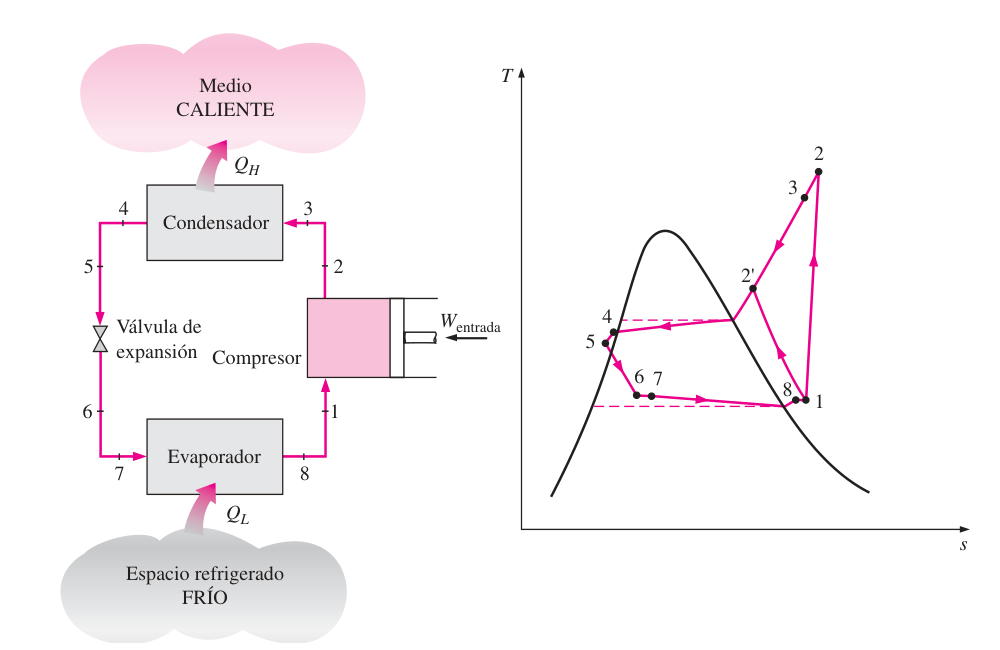
\includegraphics[width=\linewidth]{figures/diag-ts}
	\caption{Diagrama T-S del ciclo de refrigeración}
	\label{fig:diag-ts}
	\end{figure} En este contexto, la integración de principios de ciencia de materiales y simulación térmica permite desarrollar cámaras de refrigeración más eficientes y seguras, asegurando la conservación de medicamentos críticos como la insulina en condiciones óptimas, incluso en escenarios desafiantes como los presentados por la Ciudad de México. Las simulaciones térmicas y los avances en el diseño de sistemas de refrigeración son cruciales para optimizar los procesos de conservación, mejorar la eficiencia energética y garantizar la seguridad del almacenamiento de medicamentos a largo plazo (Dincer \& Ratlamwala, 2016).

	\section{Diseño Experimental}
	La cámara propuesta tiene dimensiones de 50x60x60 cm y está diseñada para manejar una carga térmica total de 3500 BTU. El diseño se divide en tres aspectos principales: aislamiento térmico, sistema de refrigeración y pruebas experimentales (ver Figura \ref{fig:vista-camara}).


	
	\begin{figure}[H]
		\centering
		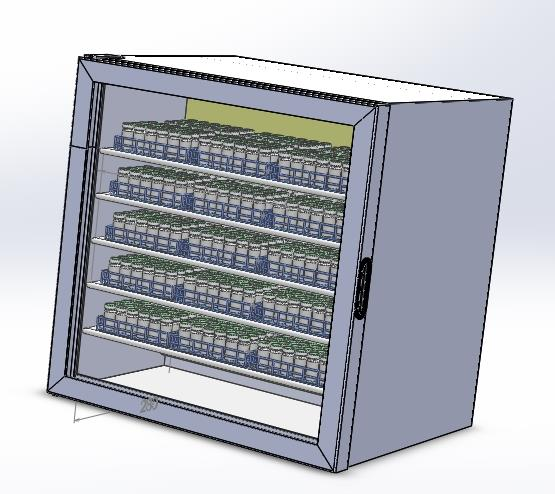
\includegraphics[width=\linewidth]{figures/axo-parrilasycharolas}
		\caption{Vista general de la cámara de refrigeración}
		\label{fig:vista-camara}
	\end{figure}
	
	
	
	\subsection{Cálculo de la Carga Térmica}
	El cálculo de la carga térmica considera tanto la transferencia de calor a través de las paredes de la cámara como las cargas internas generadas por los ocupantes y equipos. La ecuación principal se basa en el principio de conducción térmica, donde el coeficiente de transmisión térmica ($U$) y el área de aislamiento ($A$) determinan cuánto calor se transfiere entre el interior y el exterior de la cámara debido a la diferencia de temperatura. Las cargas adicionales, como las generadas por ocupantes y equipos, también se incluyen en el cálculo, aunque en este caso son consideradas negligibles.
	\color{blue}
\begin{equation}
	Q = U \cdot A \cdot (T_{\text{int}} - T_{\text{ext}}) + Q_{\text{ocupantes}} + Q_{\text{equipos}} 
\end{equation}
\color{black}
	
	donde:
	\begin{itemize}[itemsep=0.25em, topsep=0.25em, partopsep=0pt]
		\item $Q$: carga térmica total (BTU).
		\item $U$: coeficiente de transmisión térmica del material (BTU/h-ft$^2$-$^\circ$F).
		\item $A$: área total del aislamiento (ft$^2$).
		\item $T_{\text{int}}$ y $T_{\text{ext}}$: temperaturas interior y exterior ($^\circ$F).
		\item $Q_{\text{ocupantes}}$: carga generada por ocupantes (negligible en este caso).
		\item $Q_{\text{equipos}}$: carga generada por equipos internos (negligible).
	\end{itemize}
	
	Para materiales con $U$ bajo (como el poliuretano expandido), se reduce significativamente la transferencia de calor, como se muestra en la Tabla \ref{tab:materiales}.
	
 	
	
\begin{table}[H]
	\centering
	\caption{Comparación de Materiales de Aislamiento Térmico} 
	\label{tab:materiales}
\begin{tabular}{|p{2cm}|p{4cm}|}
	\hline
	\textbf{Material} & \textbf{Propiedades} \\ \hline
	\textbf{Poliuretano Expandido} & Conductividad térmica: 0.02 W/mK \\ \hline
	\textbf{Acero Inoxidable} & Alta resistencia a la corrosión. \\ \hline
	\textbf{Juntas de Silicona} & Material flexible, alta capacidad de sellado \\ \hline
\end{tabular}
	\vspace{0.11cm} % Espacio entre la tabla y la sección de Ventajas
	
	\begin{tabular}{|l|}
		\hline
		\textbf{Ventajas} \\ \hline
		Excelente aislamiento con espesores pequeños \\ \hline
		Durabilidad y resistencia a ambientes agresivos \\ \hline
		Garantiza hermeticidad y previene pérdidas térmicas \\ \hline
	\end{tabular}
\end{table}




\subsection{Selección de Materiales}
A continuación se propone una selección de materiales clave para el diseño y construcción de la cámara de refrigeración, considerando sus propiedades térmicas, mecánicas y de durabilidad para garantizar un rendimiento eficiente y confiable en condiciones operativas exigentes (Área de teconologia, 2016). 

\begin{itemize}[itemsep=0.25em, topsep=0.25em, partopsep=0pt]
	\item \textbf{Aislamiento térmico:} Poliuretano expandido con una conductividad térmica de 0.02 W/mK, que ofrece un excelente aislamiento con espesores pequeños.
	\item \textbf{Recubrimientos internos y externos:} Acero inoxidable, elegido por su resistencia a la corrosión y facilidad de limpieza.
	\item \textbf{Sellado:} Uso de juntas de silicona para garantizar hermeticidad y prevenir pérdidas térmicas.
	\item \textbf{Resistencia mecánica:} Materiales que soporten impactos y vibraciones sin comprometer la estructura, asegurando que la cámara mantenga su integridad durante largos periodos de uso.
	\item \textbf{Durabilidad a largo plazo:} Selección de materiales resistentes a la degradación por factores como la humedad, la radiación UV y los ciclos térmicos, garantizando que la cámara continúe funcionando de manera óptima durante su vida útil.
\end{itemize}
	
 \begin{figure}[H]
 	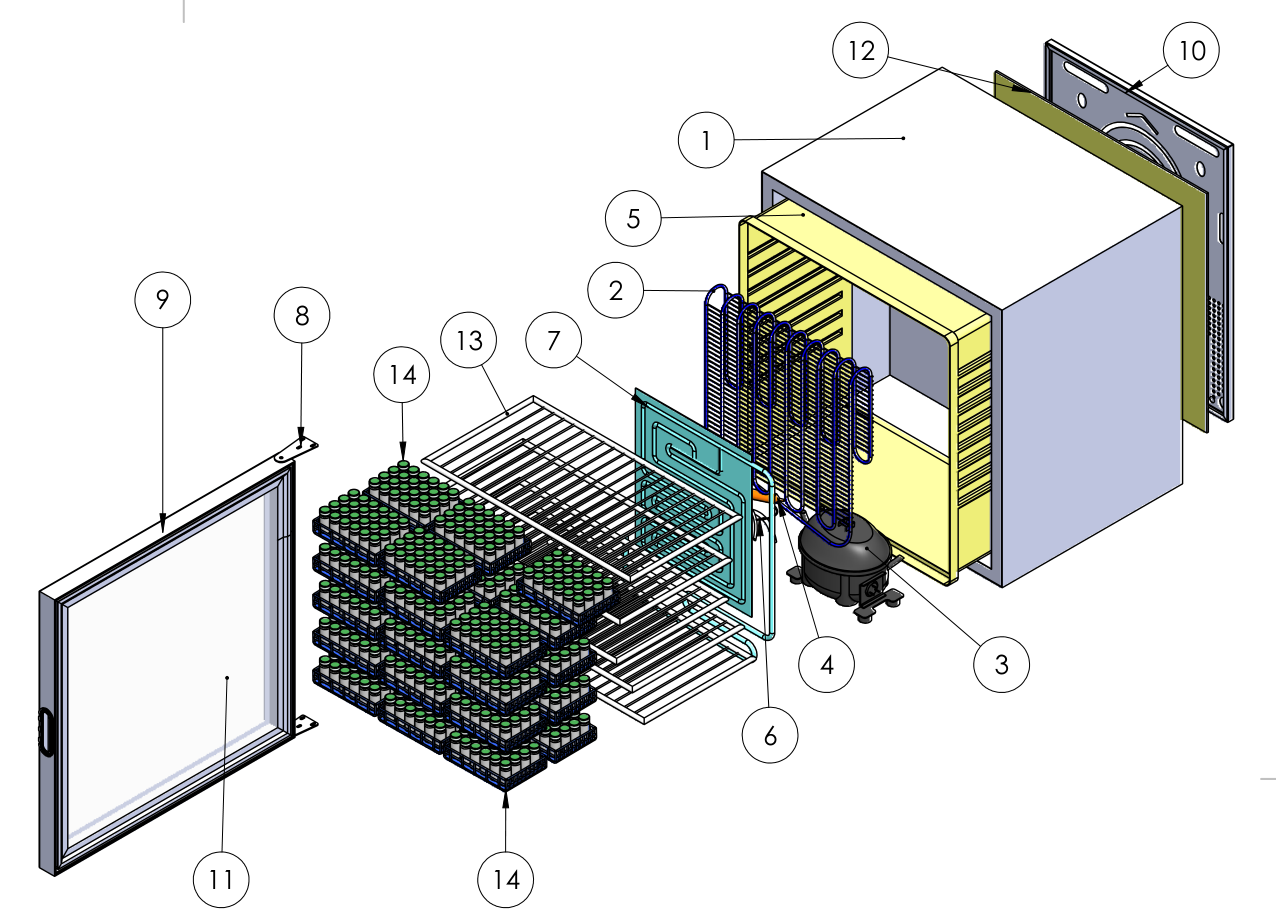
\includegraphics[width=\linewidth]{figures/front-chapetr4.png}
 	\caption{Equipo de refrigeración diseñado}
 \end{figure}
 
	\subsection{Simulación y Evaluación de Materiales}
	Para validar el diseño, se realizaron simulaciones térmicas usando software como ANSYS, evaluando la distribución de temperatura y el flujo de calor. Además, se realizaron pruebas de impacto para garantizar que el recubrimiento resista deformaciones (ver Figuras  \ref{fig:dist-intcalor} y  \ref{fig:temp-simulation}).
	

 \begin{figure}[H]
 	\centering
 	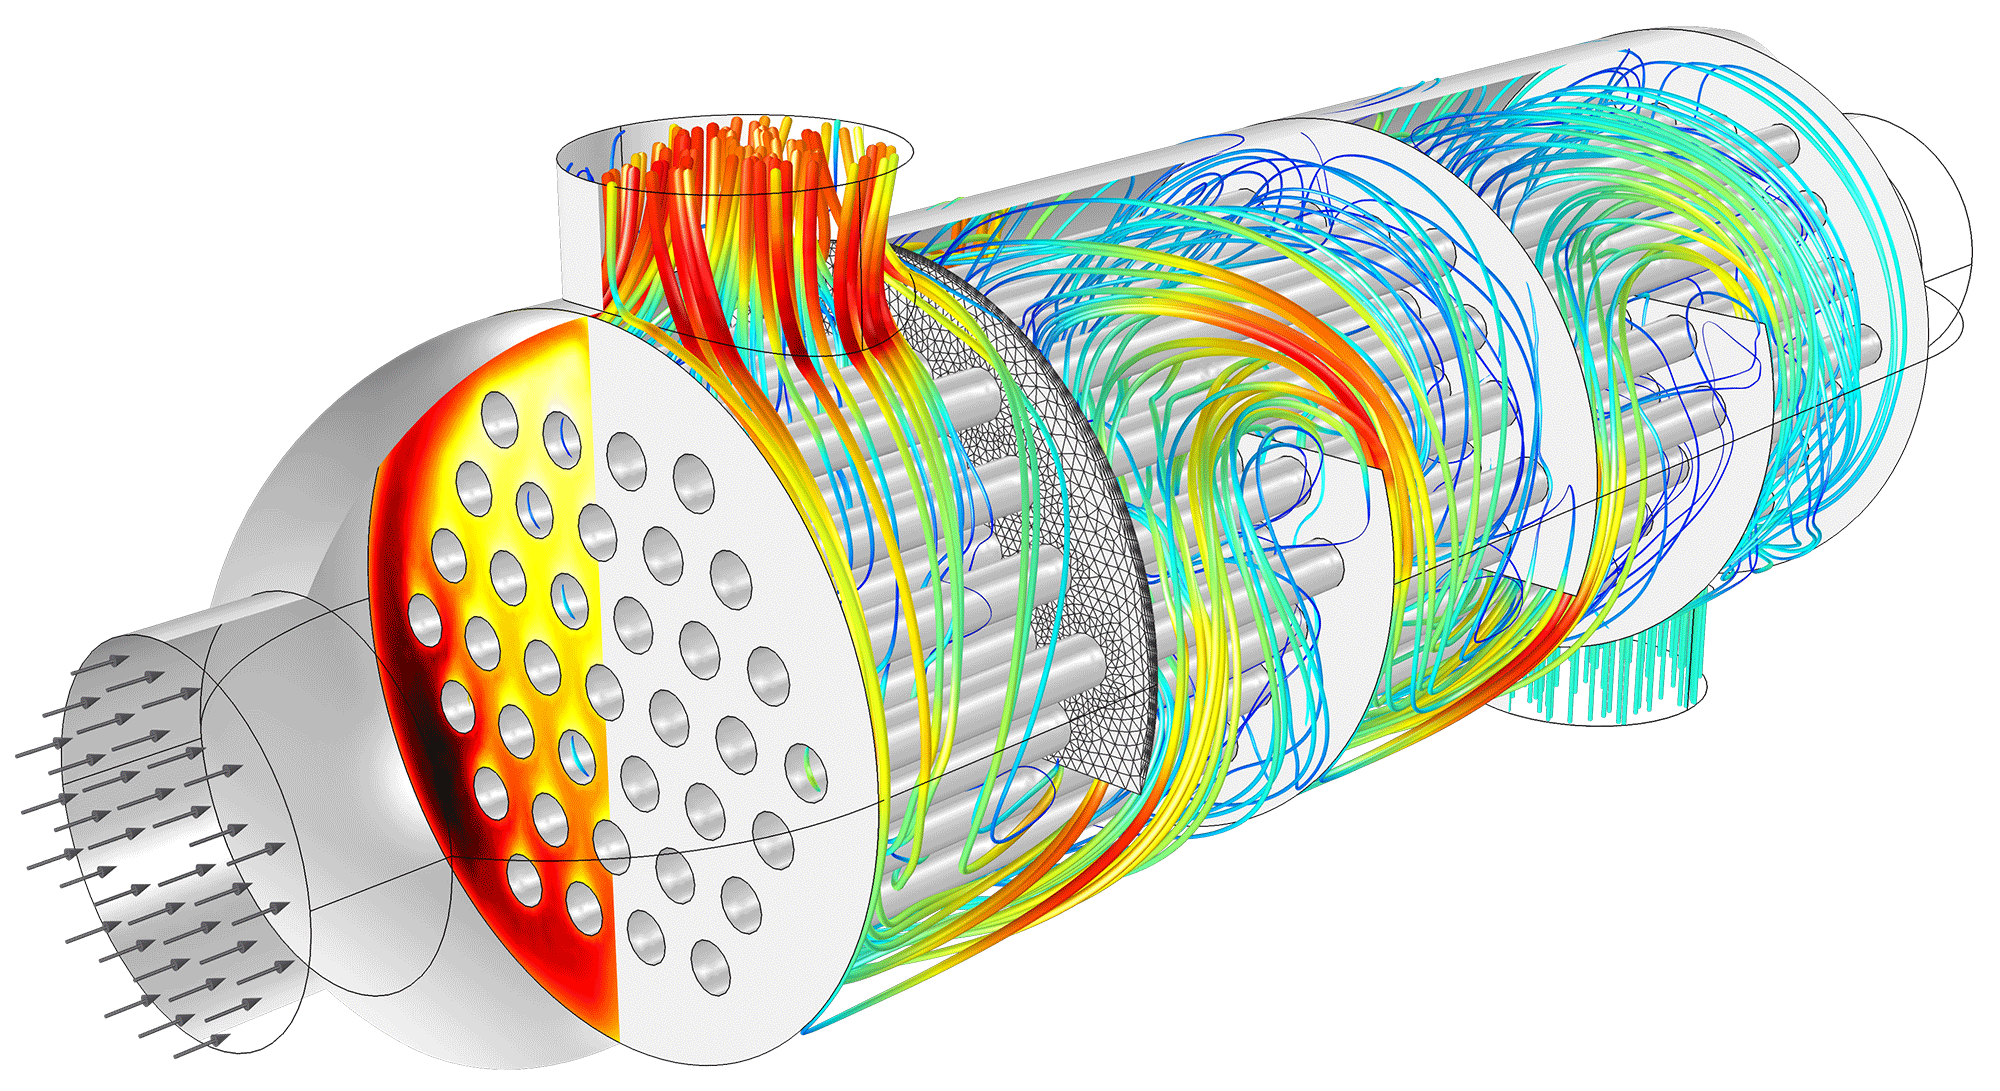
\includegraphics[width=\linewidth]{figures/dist-intcalor}
 	\caption{Simulación de intercambiador de calor.}
 	\label{fig:dist-intcalor}
 \end{figure}
 
 	\begin{figure}[H]
		\centering
		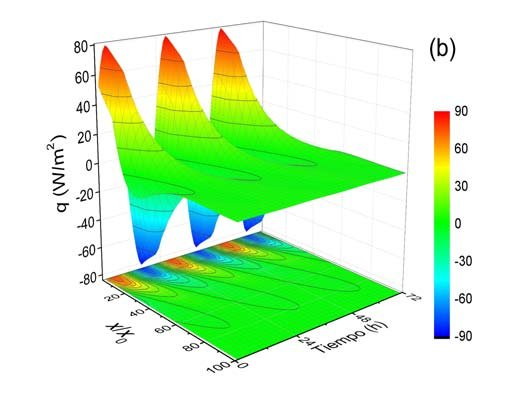
\includegraphics[width=\linewidth]{figures/temp-simulation}
		\caption{Distribución espacio-temporal del flujo de calor por unidad de área, en función del tiempo.}
		\label{fig:temp-simulation}
	\end{figure}
	
	
\section{Resultados y Discusión}
\textbf{Eficiencia Energética}: El sistema diseñado mantiene una temperatura estable de $4^\circ$C con un consumo energético optimizado. Las simulaciones térmicas realizadas muestran que el poliuretano expandido reduce las pérdidas térmicas en un 30\% en comparación con materiales tradicionales, lo que demuestra su efectividad en mantener las condiciones térmicas estables con un menor gasto energético. Este resultado es fundamental para garantizar la eficiencia operativa y la reducción de costos a largo plazo.

\textbf{Impacto de la Altitud}: La altitud, que disminuye la presión del aire, afecta directamente la capacidad del condensador y el compresor, lo que podría comprometer la eficiencia del sistema de refrigeración. Sin embargo, el condensador modelo CH111*B - CH501*B de temperatura baja ha demostrado ser capaz de compensar adecuadamente estas pérdidas. Las pruebas realizadas bajo condiciones simuladas de altitud mostraron que el sistema mantiene un rendimiento eficiente, adaptándose bien a las condiciones específicas de la Ciudad de México, que se encuentra a 2250 metros sobre el nivel del mar.

\textbf{Pruebas de Resistencia}: Las pruebas de resistencia realizadas confirmaron la durabilidad y la funcionalidad de la cámara bajo diversas condiciones de operación, evaluando tanto los recubrimientos externos como el aislamiento térmico. Estas pruebas fueron diseñadas para simular escenarios reales de uso intensivo, como caídas accidentales o golpes que podrían producirse en entornos médicos. Los resultados demostraron que los materiales utilizados son capaces de resistir estos desafíos, asegurando que la cámara mantenga su integridad estructural a lo largo de su vida útil. 

En las pruebas de impacto mecánico, se evaluó la resistencia de los recubrimientos de acero inoxidable frente a impactos accidentales y vibraciones típicas en entornos médicos. Se utilizaron análisis de elementos finitos (FEM) en ANSYS, aplicando cargas puntuales y distribuidas que representaban golpes comunes, como los causados por equipos rodantes o caídas de objetos. Los resultados mostraron que el recubrimiento de acero inoxidable puede soportar fuerzas de hasta 50 N sin sufrir deformaciones permanentes, lo que garantiza que la cámara podrá operar de forma segura en ambientes exigentes.

Se realizaron pruebas de presión interna para verificar la hermeticidad del sistema. La cámara fue sometida a variaciones de presión interna, simulando el cierre brusco de la puerta. Los sellos de silicona utilizados en la cámara demostraron su efectividad, ya que evitaron fugas de aire incluso después de 10,000 ciclos de apertura y cierre, lo que asegura la estabilidad térmica en su interior durante su vida útil.

En cuanto a las pruebas de ciclos térmicos, el aislamiento térmico de poliuretano expandido fue evaluado mediante ciclos de calentamiento y enfriamiento entre $-5^\circ$C y $40^\circ$C, reproduciendo escenarios extremos de operación. Las pruebas revelaron que el aislamiento mantiene su rendimiento térmico incluso después de más de 500 ciclos, sin evidencias de degradación significativa. Este comportamiento valida la durabilidad del material, asegurando que mantendrá su capacidad aislante incluso bajo condiciones térmicas fluctuantes.

Además, se llevaron a cabo pruebas de envejecimiento acelerado exponiendo los materiales a humedad relativa del 60 al 90\% y temperaturas constantes de 23 al $30^\circ$C durante un periodo simulado de 5 años. Los resultados indicaron que tanto los recubrimientos como los sellos de silicona y el aislamiento térmico mantienen más del 92.3\% de sus propiedades originales después del periodo de simulación, lo que garantiza su funcionalidad a largo plazo, incluso en condiciones ambientales extremas.

Finalmente, se realizaron pruebas de carga estructural para evaluar la capacidad de la cámara para soportar cargas estáticas y dinámicas, como el peso de equipos médicos colocados sobre su superficie. Los análisis confirmaron que la estructura puede soportar hasta 30 kg sin deformaciones significativas, proporcionando una base sólida para su integración en hospitales o clínicas, donde el equipo puede estar sujeto a impactos o cargas externas durante su uso.
	
	\section{Conclusión}
El diseño y la selección de materiales para la cámara de refrigeración propuesta se fundamentan en principios avanzados de ingeniería térmica, confiabilidad estructural y durabilidad, adaptados a las condiciones ambientales específicas de la Ciudad de México. La elección del poliuretano expandido como material de aislamiento, junto con el acero inoxidable para recubrimientos, asegura no solo un aislamiento térmico de alto rendimiento, sino también resistencia a factores externos como la corrosión y la abrasión, lo cual es esencial en entornos médicos rigurosos.

El uso de simulaciones térmicas avanzadas mediante ANSYS permitió optimizar el diseño y validar la eficiencia energética del sistema, garantizando un consumo energético reducido sin comprometer la capacidad de refrigeración. Las pruebas realizadas confirmaron que la cámara mantiene una temperatura estable de $4^\circ$C, con una reducción significativa de las pérdidas térmicas, lo que optimiza el almacenamiento de la insulina y prolonga su vida útil.

Adicionalmente, las pruebas de resistencia mecánica, hermeticidad y durabilidad bajo condiciones extremas demostraron que la cámara puede soportar los desafíos operativos diarios en entornos hospitalarios. La capacidad del sistema para resistir impactos, variaciones de presión y ciclos térmicos asegura su fiabilidad a largo plazo. Las pruebas de envejecimiento acelerado y carga estructural corroboraron que los materiales seleccionados no solo cumplen con los requisitos de seguridad, sino que también mantienen su integridad funcional durante años de uso continuo.

El sistema de refrigeración ofrece una solución robusta y confiable para la conservación de insulina, alineada con los estándares internacionales más exigentes en la industria médica. La combinación de un diseño estructural eficiente, una selección cuidadosa de materiales y la validación mediante simulaciones avanzadas posiciona esta cámara como una herramienta crítica para garantizar la seguridad y efectividad del tratamiento para pacientes con diabetes. Este enfoque integral en la ingeniería y la ciencia de materiales no solo optimiza el almacenamiento, sino que también contribuye a la mejora en la atención médica y la preservación de medicamentos vitales.


%\bibliographystyle{apacite}
\bibliographystyle{plain}  

\bibliography{paperreferences.bib}
\begin{itemize}
	\setlength\itemindent{-1em} % Define la sangría francesa
	\setlength{\leftskip}{1em}  % Ajusta la sangría para el resto de las líneas
	%\item[] Dincer, I., \& Ratlamwala, T. A. H. (2016). \textit{Integrated Absorption Refrigeration Systems}. Springer.
	\item[] Cengel, Y. A. (2009). \textit{Introduction to Thermodynamics and Heat Transfer}. McGraw-Hill. 
	\item[] Kaushik, S. C. (2017). \textit{Finite Time Thermodynamics of Power and Refrigeration Cycles}. Springer
	\item[] Zhang, X. R., \& Eikevik, T. M. (2023). \textit{CO2 Refrigeration Cycle and Systems}. Springer Nature.  
	 
\end{itemize}

\end{multicols}



\end{document}
